\documentclass[handout]{beamer}
\RequirePackage[italian]{babel}
\RequirePackage[utf8]{inputenc}

\RequirePackage{amsmath}
\RequirePackage{dsfont}
\RequirePackage{mathtools}
\RequirePackage[linesnumbered,lined,ruled,vlined,commentsnumbered]{algorithm2e}

\RequirePackage[
  backend=bibtex,
  citestyle=authoryear,
  style=alphabetic
]{biblatex}
\addbibresource{bibliography.bib}

\RequirePackage{xcolor}

\RequirePackage{pgfpages}
\setbeamertemplate{note page}[plain]
%\setbeameroption{show notes on second screen=bottom}
%\pdfinfo{/Keywords (SP-Bottom)}

\RequirePackage{minted}
\newcommand{\ipy}[1]{\mintinline{python3}{#1}}

\usetheme{Madrid}
\usecolortheme{seahorse}
\setbeamercovered{transparent}

\RequirePackage{minted}
\usemintedstyle{github}

\RequirePackage{bm}
\renewcommand{\vec}[1]{\bm{#1}}

\RequirePackage[separate-uncertainty = true]{siunitx}

\title[Playing \emph{Connect-4} with DNN]{Playing \emph{Connect-4} with Deep Neural Networks}
\subtitle{}
\author[Luca Arnaboldi]{Luca Arnaboldi}      
\institute[]{Corso ``Computing Methods for Experimental Physics and Data Analysis''}
\date[14-10-2021]{14 ottobre 2021}

\begin{document}
  \frame[plain,noframenumbering]{\titlepage}
  
  \begin{frame}
    \frametitle{Introduzione}
    \begin{columns}
      \column{0.3\textwidth}
        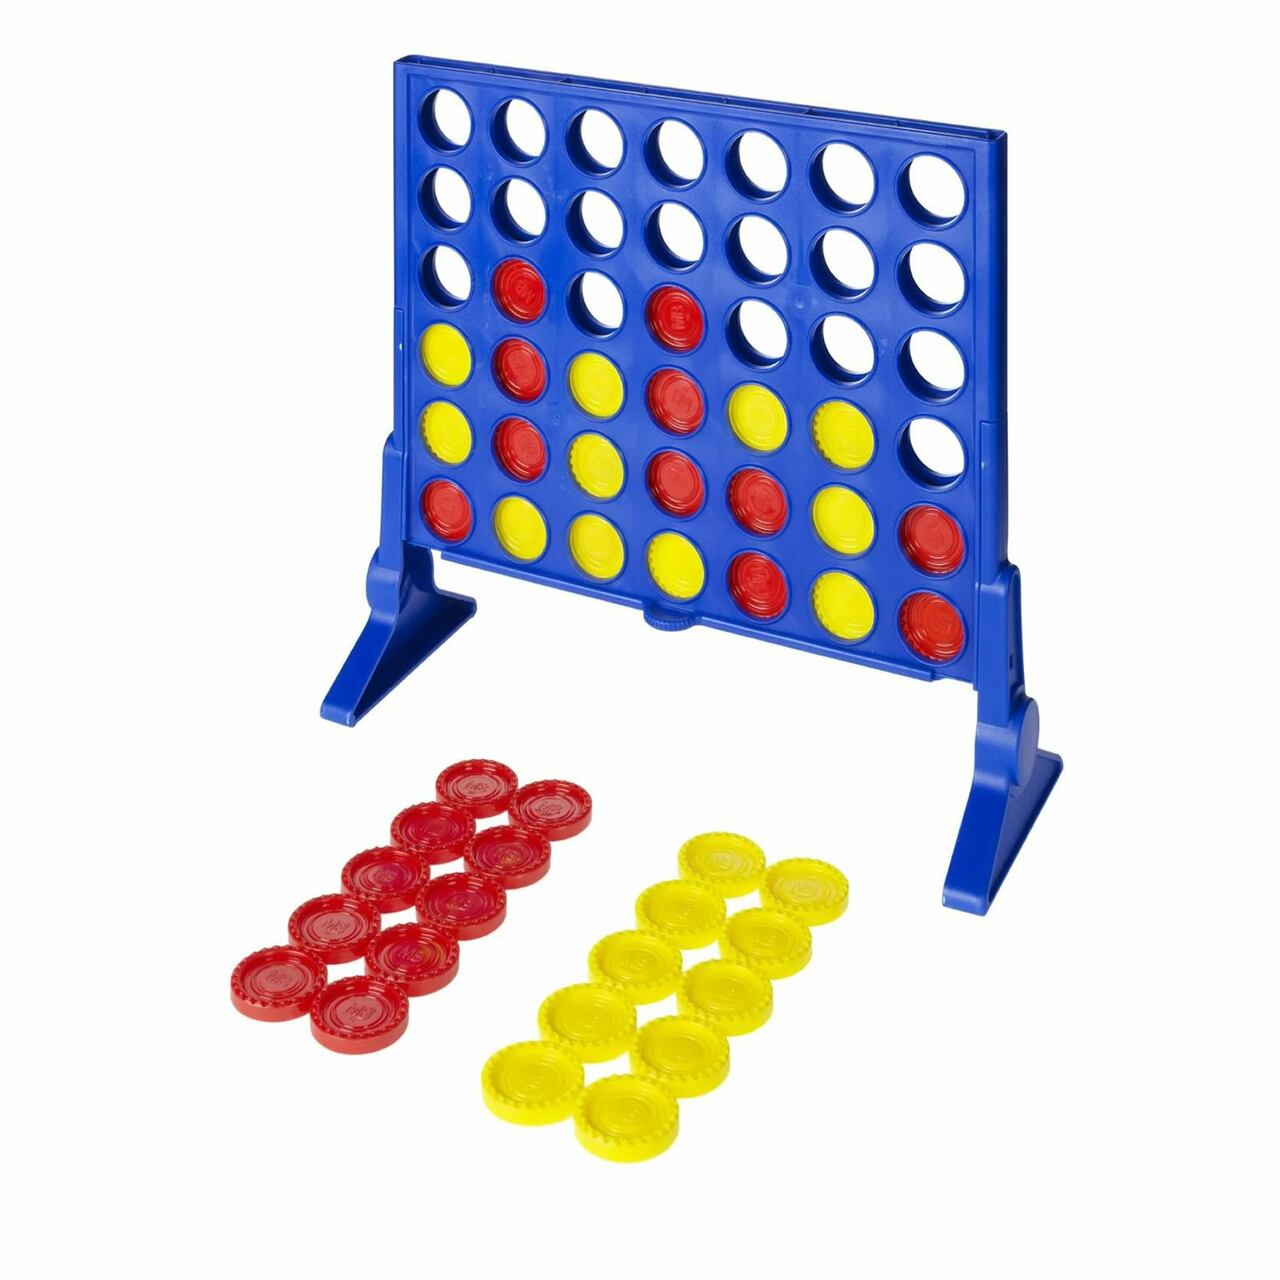
\includegraphics[width=\textwidth]{img/connect4tablegame.jpg}
      
      \column{0.7\textwidth}
        \begin{itemize}
          \item \emph{Forza-4} è un gioco ad informazione completa, con \num{4531985219092} stati possibili \cite{oeis}. 
          \item Il numero di stati limitato permette di risolvere il gioco con algoritmi di ricerca completa.
          \item Non è un problema in cui le reti neurali sono utili ai fini pratici.
        \end{itemize}      
    \end{columns}
    \pause
    È una buona palestra per testare l'abilità delle DNN, potendo fare un confronto con gli algoritmi classici. Seguiamo due approcci:
    \begin{itemize}
      \item \structure{Supervised Learning}: gli algoritmi classici generano il dataset per allenare la rete;
      \item \structure{Reinforcement learning}: il giocatore basato sulla rete neurale gioca contro se stesso ed impara dalle proprie mosse. 
    \end{itemize}
  \end{frame}

  \note{
    ``Questa è veloce una presentazione del progetto, se vogliamo scendere nel dettaglio guardiamo insieme la repo''
  }

  \begin{frame}
    \frametitle{Motore di gioco}
    Ho implementato in \texttt{Python3} il motore di gioco.\\
    Paradigma ad oggetti, uno per ogni componente fondamentale del gioco:
    \begin{itemize}
      \item \ipy{Board}: tavola di gioco, contenente tutti i metodi necessari per aggiungere/togliere pedine, calcolare il vincitore e validare le configurazioni di gioco.
      \item \ipy{Game}: classe che gestisce una partita tra due giocatori. Gestisce l'alternanza dei turni e in generale regola il l'ordine con cui vengono chiamati i metodi sugli oggetti \ipy{Player}.
      \item \ipy{Player}: è la classe classe base per tutti gli altri giocatori; è puramente astratta.
    \end{itemize}
    \pause
    
    Extra: classe \ipy{Tournament}, \ipy{costants}
    
    % Notes
    \note<1>[item]{\ipy{Board} è separato da \ipy{Game} perchè alcuni algoritmi hanno bisogno di una Board senza necessitare di una partita completa.}
    \note<2>[item]{\ipy{Tournament} potrebbe implementare calcolo in parallelo.}
    \note<2>[item]{\ipy{Tournament} da un sacco di statistiche utili e differenzia tra primo giocatore e secondo giocatore. INIZIARE È FORTISSIMO!!}
    \note<2>[item]{In teoria è pensato per giocare a Forza-n, su griglie generiche... Ma non ci ho mai provato}
  \end{frame}

  \begin{frame}
    \frametitle{Players}
    \begin{itemize}
      \item<1-> \structure{Basic Players}: giocatori senza una vera strategia:
      \begin{itemize}
        \item \ipy{RandomPlayer}: gioca una mossa random tra quelle consentite.
        \item \ipy{ConsolePlayer}: legge dallo \texttt{stdin} le mossa da fare.
        \item \ipy{FixedMovesPlayer}: gioca una sequenza predeterminata di mosse.
      \end{itemize}
    
      \item<2-> \structure{Search Players}: giocatori basati sull'esplorazione dell'albero delle configurazioni. Algoritmo:
      \[\text{minimax} + \text{alpha-beta pruning} + \text{euristiche}\]
      \vspace{-20pt}
      \begin{columns}
      \column{0.05\textwidth}
      \column{0.95\textwidth}
        \begin{block}<3->{\ipy{PerfectPlayer}}
          Implementazione in \texttt{C++} di una ricerca completa\cite{perfectsolvertutotial, perfectsolverimplementation}. Incluso nella repository come submodule.
        \end{block}
      \end{columns}
      \item<4-> \structure{Combination Players}: combinazione di 2 o più giocatori.
      \item<5-> \structure{TensorFlow Players}: valutazione della tavola con un modello di \textit{TensorFlow}.
    \end{itemize}
  
    % Notes
    \note<1>[item]{\ipy{FixedMovesPlayer} è usato principalmente per l'unit testing.}
    \note<2>[item]{Le euristiche sono l'ordine in un caso e il rumore nell'altro}
    \note<4>[item]{I giocatori di combinazione sono il \ipy{TwoStagePlayer} e \ipy{PoolPlayer}.}
  \end{frame}

  \begin{frame}
    \frametitle{Extras}
    \begin{itemize}
      \item \structure{Testing}: \texttt{PyTest}
      \item \structure{Linting}: \texttt{Flake8}
      \item \structure{Documentazione}: \texttt{Sphinx}
      \item \structure{Continuous Integration}: \texttt{GitHub Workflows}
      \item \structure{Continuous Deployment}: \texttt{GitHub Pages}  
    \end{itemize}
    \begin{figure}
      
\includegraphics[width=0.8\textwidth]{img/github_badges.png}
    \end{figure}
    \begin{center}
      \url{https://arn4.github.io/connect4/}
    \end{center}
  \end{frame}

  \note{
    ``È una pagina creata in automatico dal README.md''
  }

  \begin{frame}
    \frametitle{Codice d'esempio}
    \inputminted[fontsize=\scriptsize]{python3}{code/example-game.py}
  \end{frame}

  \begin{frame}
    \begin{columns}
      \column{0.5\textwidth}
        \centering
        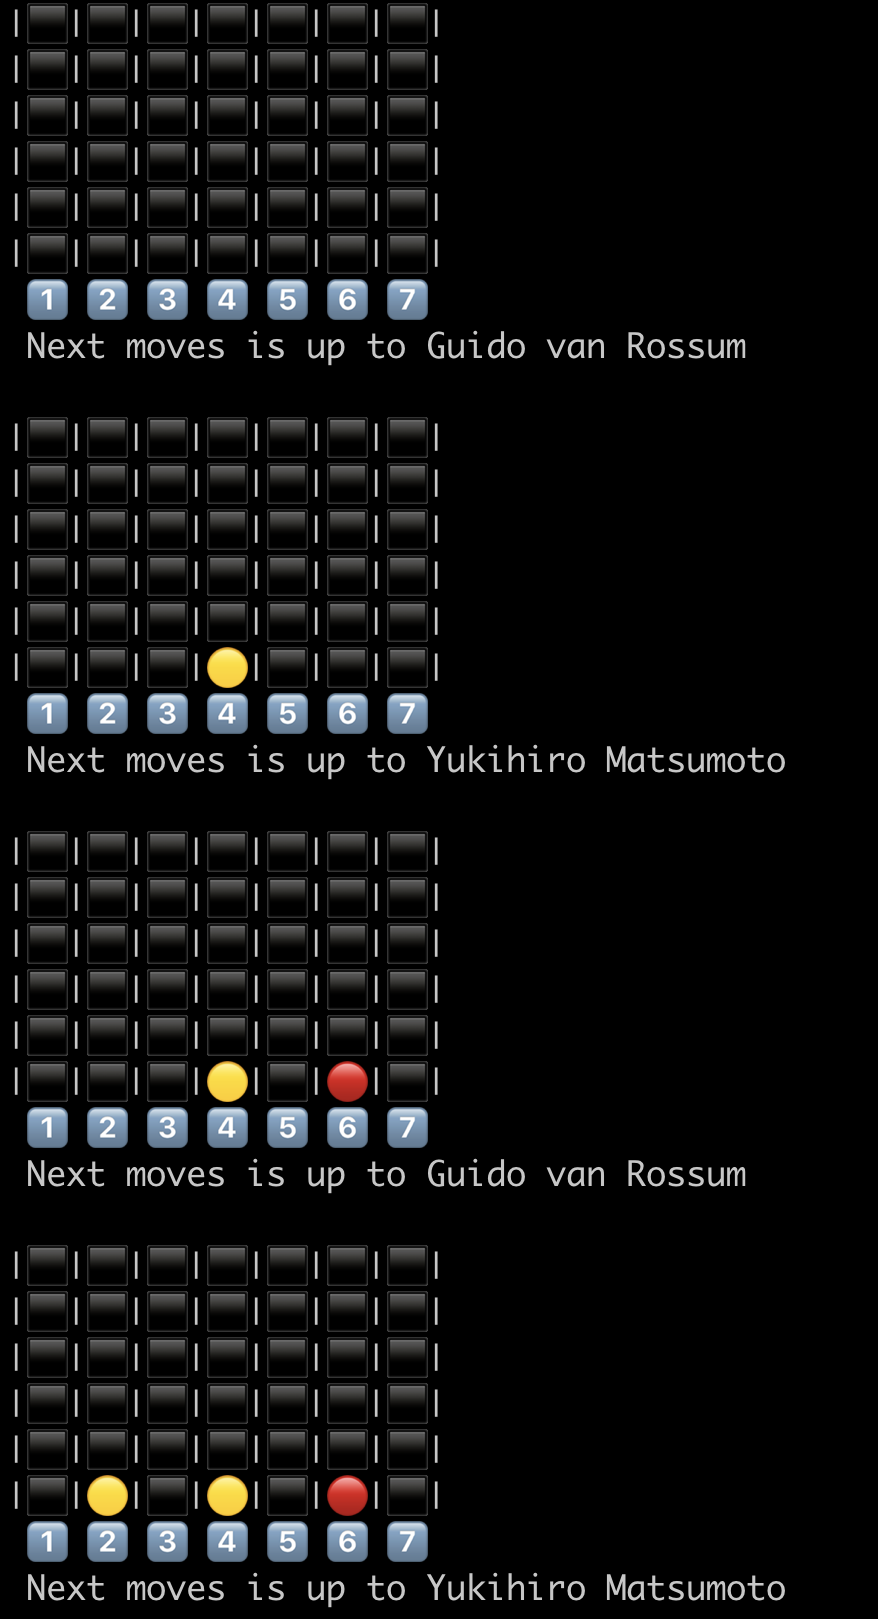
\includegraphics[width=0.8\textwidth]{img/gamestart.png}
      \column{0.5\textwidth}
        \centering
        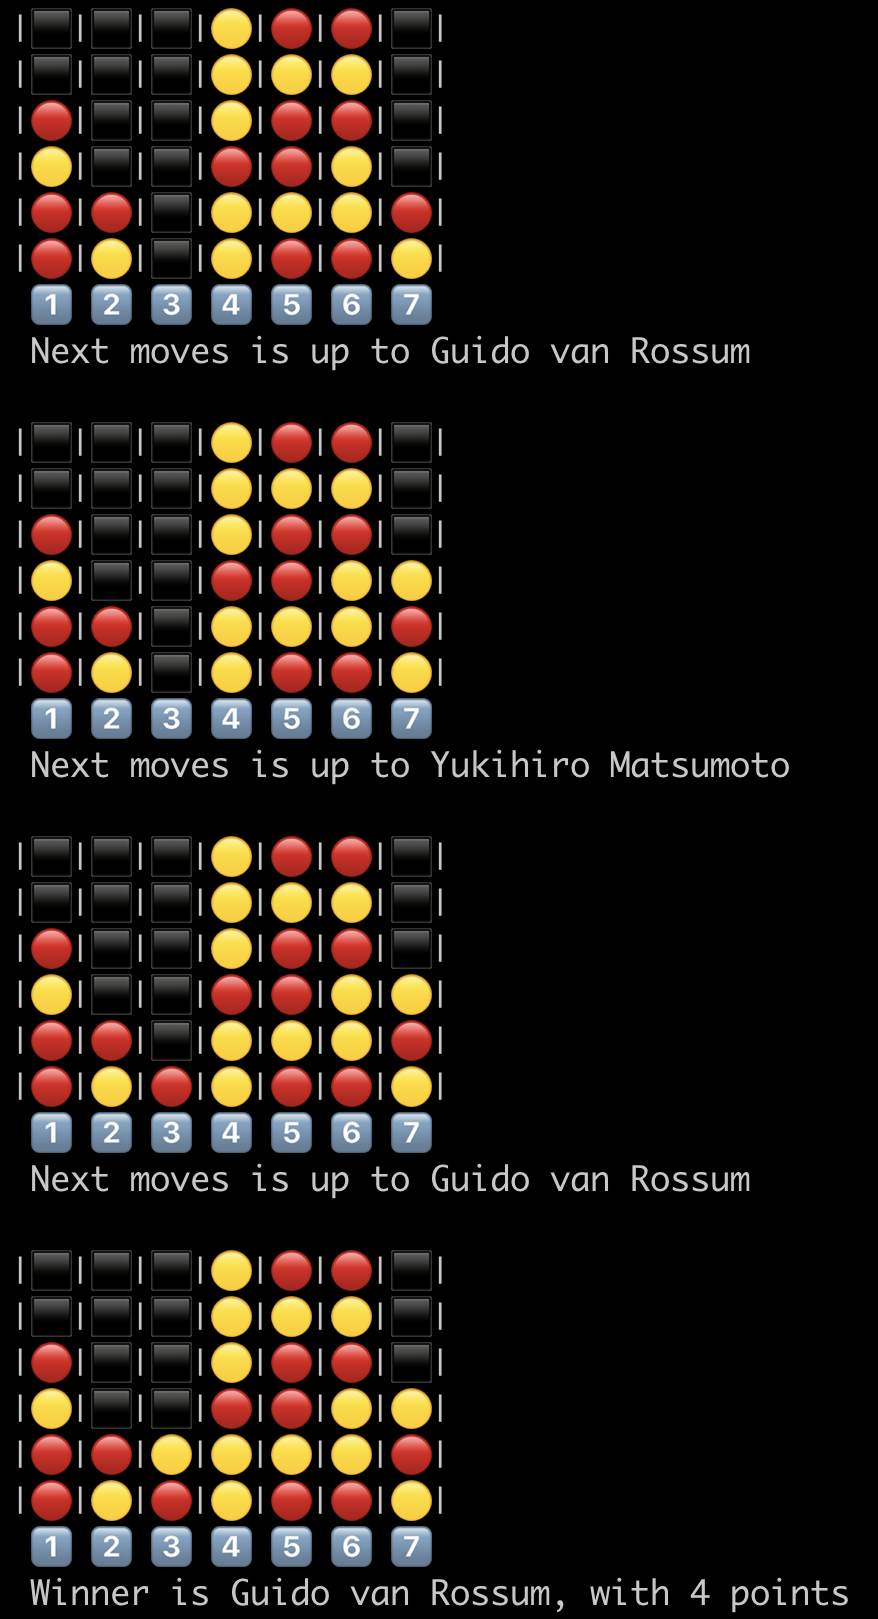
\includegraphics[width=0.8\textwidth]{img/gameend.png}
    \end{columns}
  \end{frame}

  \begin{frame}
    \frametitle{Supervised Learning: creazione del training set}
    \[
      \text{\ipy{GameEngine.Game}}
      \xrightarrow[\text{derivata}]{\text{classe}}
      \text{\text{\ipy{SupervisedGame}}}
    \]
    
    Oltre ad i due giocatori c'è un \emph{supervisor}, che in ogni situazione di gioco dice la mossa che avrebbe fatto.
    \pause
    
    \vspace{10pt}
    \structure{\ipy{DatasetGenerator}} gioca in \emph{parallelo} tante partite supervised e ritorna un dataset in formato \texttt{numpy.array}
    \pause
    
    \vspace{10pt}
    \structure{Il dataset che ho generato}
    \vspace{5pt}
    \begin{columns}
      \column[t]{0.45\textwidth}
        Giocatori:
          \begin{itemize}
            \item \ipy{RandomPlayer}
            \item \ipy{NoisyAlphaBetaPlayer} con diversi rumori e profondità.
          \end{itemize}
      \column{0.3\textwidth}
        Supervisor: \ipy{CenteredAlphaBeta} con \texttt{depth = 6} 
      \column{0.2\textwidth}
        \num{42000} partite
    \end{columns}
  
    % Notes
    \note<2>[item]{In parallelo significa \ipy{multiprocessing.Pool}}
  \end{frame}

  \begin{frame}
    \frametitle{Supervised Learning: topologia della rete}
    \begin{itemize}
      \item Il problema ha già una struttura 2D: \emph{convolutional neural network}.
      \item Kernel quadrati di dimensione 4. Uso \emph{padding valid}.
      \item I layer che dunque ho usato sono:
        \begin{itemize}
          \item Convolutional Layer con 100 feature
          \item Flatten Layer
          \item Dense Layer con 50 neuroni, \texttt{ReLU}
          \item Dense Layer con 50 neuroni, \texttt{ReLU}
          \item Dense Layer con 7 neuroni come output. Sono i \emph{logits} delle probabilità che quella sia la miglior mossa.
        \end{itemize}
      \item Loss function: \emph{Binary Crossentropy}
      \item Adam Optimizer
    \end{itemize}
  
    % Notes
    \note[item]{Binary crossentropy: \[-\frac1{N_\text{batch}}\sum_i^{N_\text{batch}} \sum_j^{N_\text{COL}}y_{ij} \log p_{ij},\] \(y\) quello del dataset, \(p\) la predizione della mia rete.}
  \end{frame}

  \begin{frame}
    \frametitle{Supervised Learning: pulizia del dataset}
    Possibili correzioni che si possono applicare al dataset:
    \begin{itemize}
      \item \structure{Simmetria longitudinale}: la tavola è simmetrica per riflessione rispetto alla colonna centrale.
      \item \structure{Duplicati}: alcune configurazioni possono essere duplicate nel dataset, si possono rimuovere.
      \item \structure{Informazione minima}: il supervisore potrebbe non essere in grado di fornire informazione sufficiente su alcune configurazioni, che dunque si possono scartare.
    \end{itemize}
    \pause
    \vspace{20pt}
    Alleno la rete per 300 epoche, con diverse combinazioni delle correzioni.
  \end{frame}

  \begin{frame}
    \frametitle{Supervised Learning: risultati}
    \begin{figure}
      \centering
      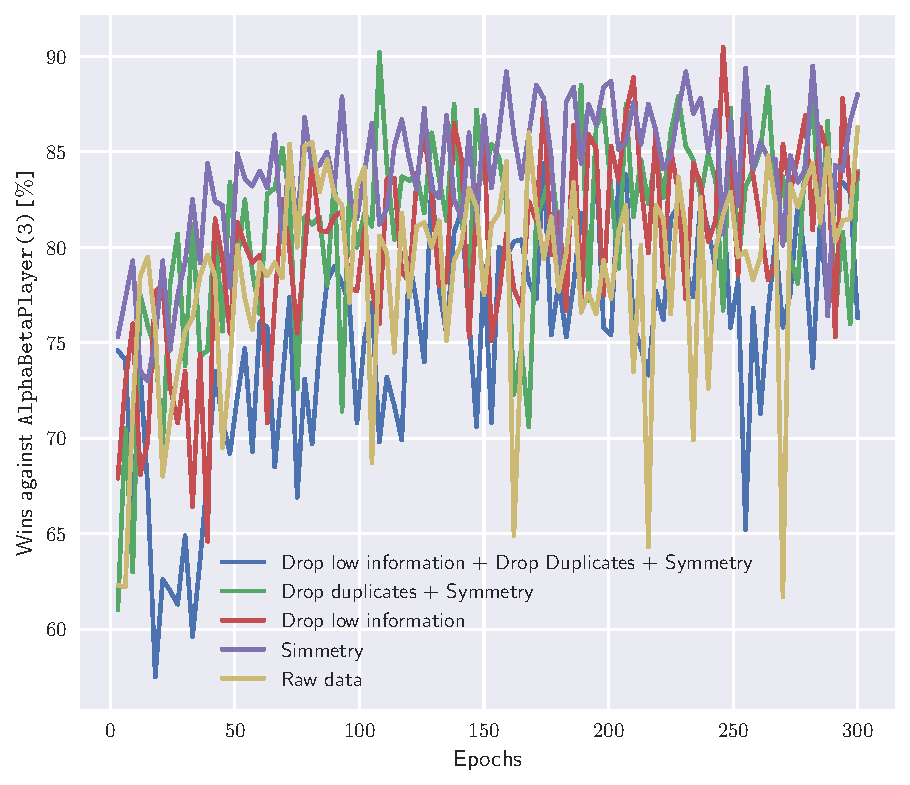
\includegraphics[width=0.77\textwidth]{img/supervised.pdf}
    \end{figure}
  
   % Notes
    \note[item]{Ho usato il \ipy{TwoStagePlayer} per randomizzare, dato che tutti questi giocatori sono deterministici.}
    \note[item]{Generare questo grafico richiede 36 ore!}
    \note[item]{Sembra che la simmetria funzioni, il resto non tanto.}
  \end{frame}

  \begin{frame}
    \frametitle{Supervised Learning: conclusioni}
    \begin{itemize}
      \item Usare la simmetria è una buona idea, le altre correzioni invece non lo sono.
      \item Confronto con il supervisore: \(15.4\si{\percent}\) di vittorie (su 1000 giocate).\\
            Il supervisore è al livello di un umano, ma la rete è lontana da poter competere con lui.
      \item Usare un supervisore e dei giocatori più forti sarebbe buona cosa, ma aumenterebbe esponenzialmente
            il tempo necessario per la generazione del dataset.
    \end{itemize}
    \pause
    \vspace{20pt}
    Nelle situazione reali non abbiamo possibilità di fare supervised learning.\\
    La rete deve imparare da sola: \emph{reinforcement learning}!
    
    % Notes
    \note<1>[item]{Le vittorie che ottiene sono principalmente dovute a situazioni iniziali favorevoli.}
  \end{frame}


  \begin{frame}
    \frametitle{Reinforcement learning: setup}
    \begin{columns}[t]
      \column{0.5\textwidth}
        \structure{Topologia}:
        \begin{itemize}
          \item 1 convolutional layer,\\2 hidden dense;
          \item Output layer ha un solo neurone: lo score della configurazione
          \item Loss Function: MSE
        \end{itemize}
        \pause
      \column{0.5\textwidth}
        \structure{Punteggi}:\\
        Semplificazione del \emph{deep-Q-learning}.\\
         I punteggi vengono dati a posteriori:
        \begin{itemize}
          \item \emph{vittoria}: +1
          \item \emph{sconfitta}: -1
          \item \emph{pareggio}: 0
          \item \emph{configurazione intermedie}: \(r_i = \gamma \cdot r_{i+1}\).
        \end{itemize}
    \end{columns}
   
    \pause
    \begin{columns}[t]
      \column{\textwidth}
        \structure{Trade-off Esplorazione-Apprendimento}\\
        Uso l'\emph{epsilon-greedy strategy}:
        \begin{itemize}
          \item probabilità \(\varepsilon\) di fare una mossa random invece che quella scelta dalla rete.
          \item \(\varepsilon\) decresce allo scorrere degli episodi. 
        \end{itemize}
    \end{columns}
    
  
    % Notes
    \note<2>[item]{Ho semplificato il deepQ perchè avevo bisogno di fare meno chiamate alla rete, già così è molto lento!}
    \note<2>[item]{\(\gamma\) è il \emph{reduction factor}}
  \end{frame}

  \begin{frame}
    \frametitle{Reinforcement learning: altre idee}
    \begin{itemize}
      \item \structure{Decadimento lineare}: Il decadimento di \(\varepsilon\) è solitamente scelto esponenziale. Trasformarlo in lineare potrebbe beneficiare. 
      \item \structure{Flattened NN}: potrebbe essere che non usare il convolutional layer funzioni meglio.
      \item \structure{Multi-Traning}: allenando un agent singolo potrebbe succedere che si adatti a se stesso per avere buoni punteggi. Se alleno un gruppo invece questo non dovrebbe succedere.
    \end{itemize}
    \begin{center}
      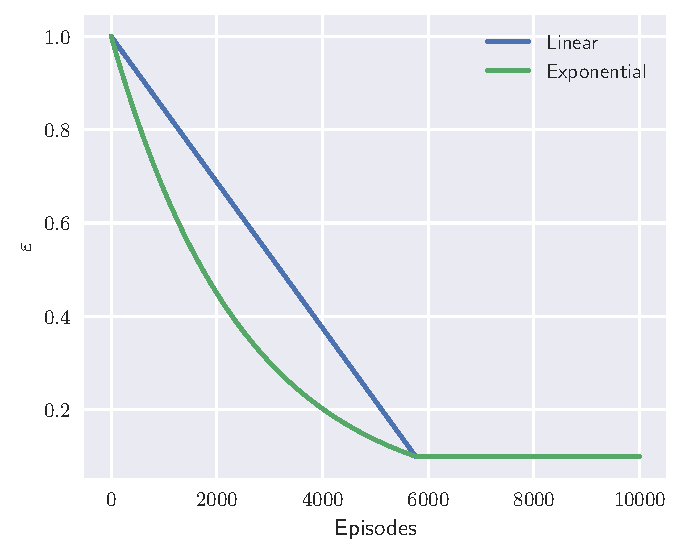
\includegraphics[width=0.46\textwidth]{img/decay.pdf}
    \end{center}
    
    % Notes
    \note[item]{Tipo un agent fatto per pareggiare sempre singolarmente sarebbe perfetto.}
  \end{frame}


  \begin{frame}
    \frametitle{Reinforcement learning: risultati preliminari}
    Alleno per \num{10000} episodi, per testare le idee
    \begin{center}
      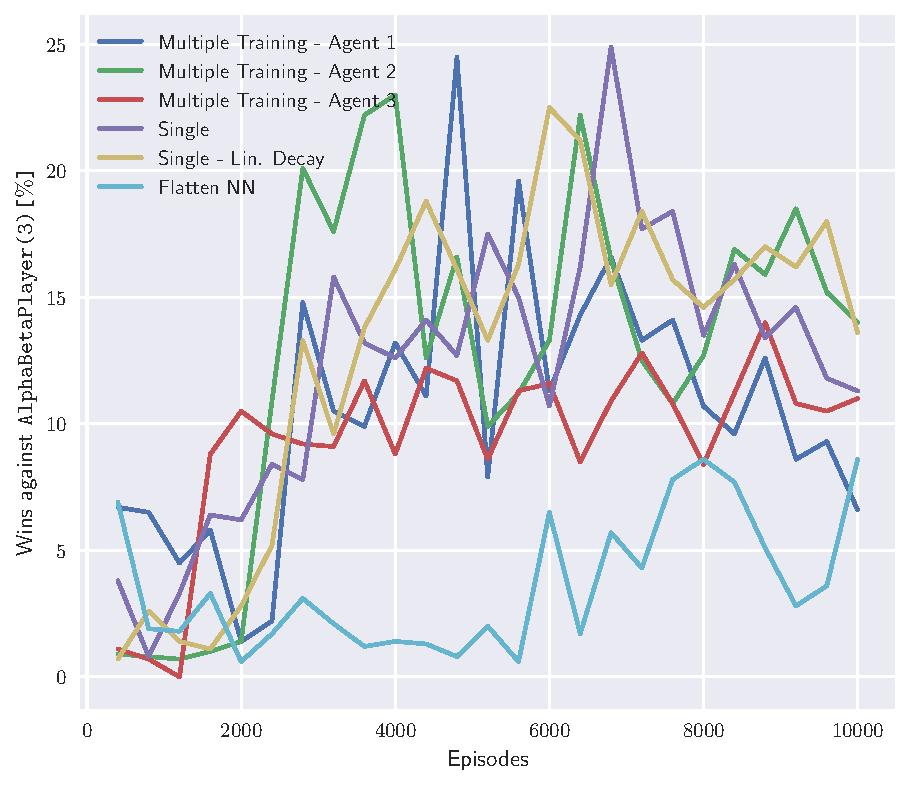
\includegraphics[width=0.7\textwidth]{img/reinforcement-10k-comparsion.pdf}
    \end{center}
  
    % Notes
    \note[item]{Solo 10000 perchè già così ci vuole infinito tempo}
    \note[item]{Fare Multi-Training non è difficoltoso, perchè tanto uso \ipy{ThreadPool}}
    \note[item]{Il decadimento lineare è più veloce, dunque lo uso}
  \end{frame}

  \begin{frame}
    \frametitle{Reinforcement learning: risultati}
    Alleno per 3 agent in simultanea, per \num{50000} episodi
    \begin{center}
      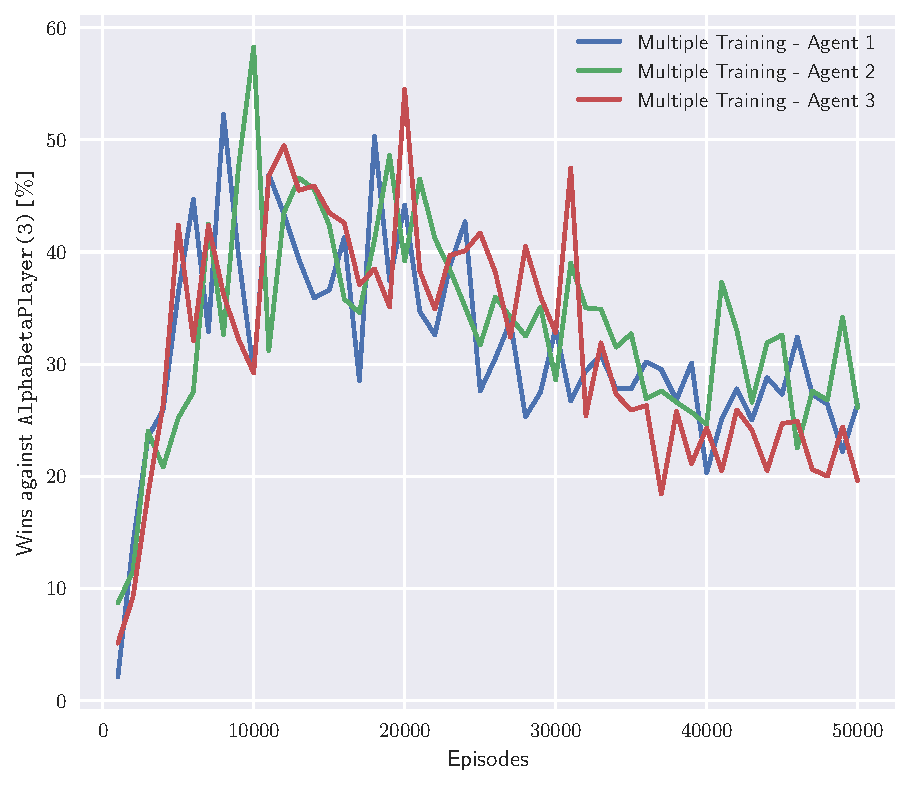
\includegraphics[width=0.7\textwidth]{img/reinforcement-50k.pdf}
    \end{center}
    
    % Notes
    \note[item]{I risultati sono lontani da quelli del supervised, ma almeno ha imparato le regole del gioco, circa}
  \end{frame}

  \begin{frame}
    \frametitle{Reinforcement learning: conclusioni}
    \begin{itemize}
      \item Prendendo la miglior performance di ognuno dei 3 agent, e combinandola in un \ipy{PoolPlayer} si ottiene \SI{57.0}{\percent} contro \ipy{AlphaBetaPlayer(3)}.
      \item La performance decresce dopo circa \num{10000} episodi: è una manifestazione del \emph{catastrophic forgetting}\cite{kirkpatrick2017overcoming}
    \end{itemize}
  
    \pause
    \begin{exampleblock}{Idea per il futuro!}
      Usare la rete neurale combinata con il \text{minimax} per avere sia la capacità di vedere il futuro che di valutare una configurazione della tavola da gioco.
    \end{exampleblock}
  \end{frame}
  


  \setbeamertemplate{page number in head/foot}{\phantom{0/0}}
  \begin{frame}[noframenumbering]
    \frametitle{Bibliografia}
    \printbibliography
  \end{frame}
  
\end{document}

